\newchapstyle
\chapter{Introduction}
\label{chap:intro}

%\epigraph[0pt]{
%    Failure is not an option.
%}{Actor Ed Harris, playing flight director Gene Kranz, in the 1995 film Apollo 13\cite{FailureNotOption2019}}

%\begin{abstract}
%Lorem ipsum dolor sit amet, consectetur adipisicing elit, sed do eiusmod tempor incididunt ut labore et dolore magna aliqua. Ut enim ad minim veniam, quis nostrud exercitation ullamco laboris nisi ut aliquip ex ea commodo consequat. Duis aute irure dolor in reprehenderit in voluptate velit esse cillum dolore eu fugiat nulla pariatur. Excepteur sint occaecat cupidatat non proident, sunt in culpa qui officia deserunt mollit anim id est laborum.
%\end{abstract}

%% Start the actual chapter on a new page.
\afterpage{\pagecolor{none}}\newpage

\section{Superconducting-normal Josephson devices}

\subsection{Andreev reflection at the SN interface}

\subsection{Andreev bound states in SNS junctions}

\begin{align}
\frac{\partial\delta}{\partial t}&=\frac{2eV_J}{\hbar}\, ,\, V_J=L_J\frac{\partial I_J}{\partial t}=L_J\frac{\partial I_J}{\partial\delta}\frac{\partial\delta}{\partial t}
\end{align}

The work done on the junction must be $U_J=\int I_J V_J {\rm d}t=\frac{\hbar}{2e}\int I_J \frac{\partial\delta}{\partial t}{\rm d}t = \frac{\hbar}{2e}\int I_J {\rm d}\delta$, therefore $I(\delta) = \frac{2e}{\hbar}\frac{\partial U_J}{\partial\delta}$.
Each Andreev bound state has a ground state energy $U_i=-\Delta\sqrt{1-T_i\sin^2(\delta/2)}$ with induced superconducting gap $\Delta$ and channel transparency $T_i$.
Summing over all of these channels, the total Josephson potential is given by
\begin{align}
U_J(\delta) &= 1-\Delta\sum_i\sqrt{1-T_i\sin^2(\delta/2)} \\
&\approx E_J \frac{\delta^2}{2} - E_J\left( 1-\frac{3\sum T_i^2}{4\sum T_i} \right) \frac{\delta^4}{24} +\mathcal{O}(\delta^6)\ , \\
E_J &= \frac{\Delta}{4}\sum_i T_i \rightarrow \frac{\Delta}{4}N\tau
\end{align}

The corresponding Josephson current and inductance are 
\begin{align}
I(\delta) &= \frac{2e}{\hbar}\frac{\partial U_J}{\partial\delta} = \frac{e\Delta}{2\hbar}\frac{\tau\sin\delta}{\sqrt{1-\tau\sin^2\delta/2}} \\
L_J(\delta) &= \frac{\hbar}{2e}\left( \frac{\partial I_J}{\partial\delta} \right)^{-1} = \left(\frac{\hbar}{2e}\right)^2\left(\frac{\partial^2U_J}{\partial\delta^2}\right)^{-1}
\end{align}

The anharmonicity in the circuit is then reduced depending on the channel transparencies.
In the limit of small $L_J$, we can model the TL resonator as a series $LC$-circuit, resulting in anharmonicity
\begin{align}
\chi &= \frac{-E_C}{2} \left( 1-\frac{3\sum T_i^2}{4\sum T_i} \right) p^3 \rightarrow \frac{-E_C}{2} \left(1-\frac{3}{4}N\tau \right) p^3 
\end{align}

\begin{figure}
	\centering
	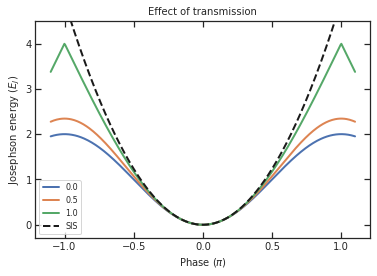
\includegraphics[width=0.7\linewidth]{chapter-introduction/figs/EJ_phase_tau}
	\caption{}
	\label{fig:ejphasetau}
\end{figure}

\begin{figure}
	\centering
	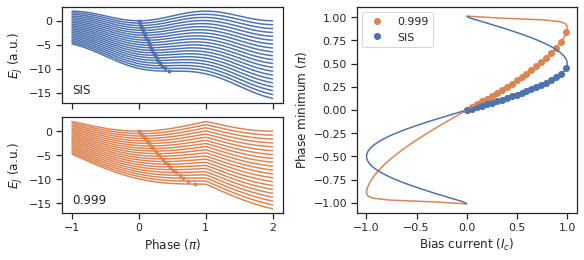
\includegraphics[width=0.7\linewidth]{chapter-introduction/figs/EJ_phase_Ib}
	\caption{}
	\label{fig:ejphaseib}
\end{figure}


\subsection{Subgap density of states}

KWANT~\cite{grothKwantSoftwarePackage2014} simulations are at \url{https://nas-steelelab.tnw.tudelft.nl:5001/?launchApp=SYNO.SDS.Drive.Application#file_id=509401234564752146}, located on the NAS under \texttt{Felix/programming/kwant}.

\subsection{The limit of low $\tau$: SIS}



\section{DC bias cavities for probing Josephson junctions}

%\subsection{Coplanar waveguide electrodynamics}

%\subsection{DC bias cavities}

In order to probe the Josephson inductance, we make use of superconducting microwave resonators based on coplanar waveguides~\cite{gopplCoplanarWaveguideResonators2008,zmuidzinasSuperconductingMicroresonatorsPhysics2012}.
%
These have been used extensively in the field of particle detection and circuit (quantum) electrodynamics due to the intrinsic low loss originating from the absence in resistance of the Cooper pairs~\cite{dayBroadbandSuperconductingDetector2003a,blaisCavityQuantumElectrodynamics2004c}.
%
In order to analyze our devices both in the low and high frequency range (DC to several $\SI{e9}{\hertz}$), our circuits need to be able to sustain relatively large quality factors while being able to introduce direct current and voltage access to the device under test (DUT).

While there is a variety of circuit architectures capable of this approach, such as using inductive coupling~\cite{vissersFrequencytunableSuperconductingResonators2015b}, direct leads at voltage nodes of a $\lambda/2$ resonator with matching length~\cite{chenIntroductionDcBias2011a,liApplyingDirectCurrent2013} or lumped-element split-cavities~\cite{mahashabdeFastTunableHigh2020}, we based our design on an architecture previously developed in our group, the shunt capacitor DC bias access~\cite{bosmanBroadbandArchitectureGalvanically2015c}.
%
The advantage of this approach is threefold:
%
As no circuit symmetries need to be considered, the design is rather simple.
%
No additional port needs to be used to probe or excite the DUT, thus there is no additional leakage channel.
%
Finally, using a shunt capacitor provides a broadband signal port up to the self-resonance of the shunt capacitor, which is chosen to be well above the resonance frequency of the circuit.

Figure~\ref{fig:DCbias} depicts a schematic of the DC bias cavity circuit.
%
In principle, measurements in both transmission and reflection geometry are possible.
%
However, we typically use the second port for supplying a DC gate voltage, and short the DUT to ground.
%
Therefore, we only perform reflection measurements.

The reflection coefficient of this circuit is given by
%
\begin{align}
S_{11}=-1+\frac{2\kappa_e}{\kappa_e+\kappa_i+2i\Delta}
\end{align}
%
with the internal and external loss rates $\kappa_i$ and $\kappa_e$ and the detuning $\Delta=\omega-\omega_0$~\cite{bosmanBroadbandArchitectureGalvanically2015c}.
%
In Fig.~\ref{fig:s11} we plot the reflection coefficient for various fractions of $\eta=\kappa_e/\kappa_i$, to illustrate the effects of over-, under- and critical coupling ($\eta>1$, $\eta<1$ and $\eta=1$, respectively).
%
For a best signal-to-noise ratio, the shunt capacitor $C_s$ should be designed such that $\kappa_e=\kappa_i$, with the external loss rate approximately given by
%
\begin{align}
\kappa_e &= \frac{\omega_0}{Q_e} = \frac{2}{\pi\omega_0Z_0^2C_s^2}
\end{align}
%
with external quality factor $Q_e$ and transmission line impedance $Z_0$.
%
However, when placing a JJ at the end of the TL, the internal loss rate can rise significantly.
%
For this reason, we typically design our circuits such that they are overcoupled without a JJ present, anticipating a rise in $\kappa_i$.

With an added Josephson junction with inductance $L_J$ shorting the TL to ground, the shifted resonance frequency can be approximated by
%
\begin{align}
\omega_0^\prime = \omega_0\frac{L_r+L_J}{L_r+2L_J}
\end{align}
%
where $L_r$ is the lumped TL resonator inductance including geometric and kinetic inductances, cf. Chapter~\ref{chap:gJJ-CPR}.


\begin{figure}
	\centering
	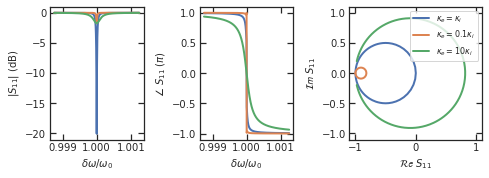
\includegraphics[width=\linewidth]{chapter-introduction/figs/S11}
	\caption{}
	\label{fig:s11}
\end{figure}


\begin{figure}
	\centering
	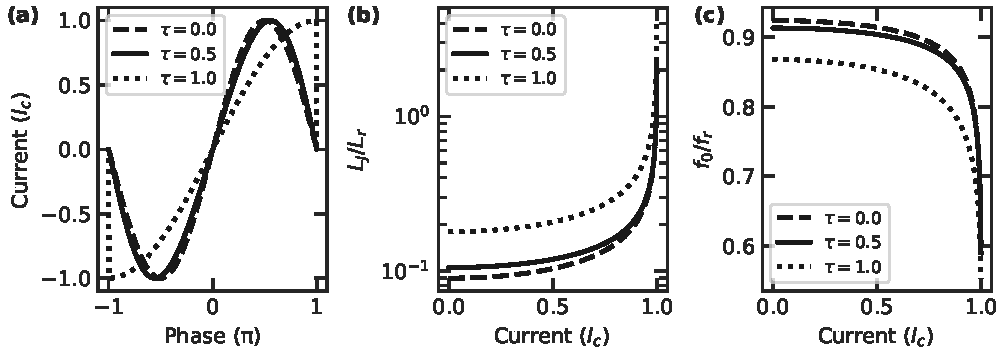
\includegraphics[width=\linewidth]{chapter-gJJ-CPR/figs/SMFigure-influence}
	\caption{}
	\label{fig:smfigure-influence}
\end{figure}


\section{Outline}
In chapter~\ref{chap:experiment}
%
In chapter~\ref{chap:gJJ}
%
In chapter~\ref{chap:gJJ-CPR}
%
In chapter~\ref{chap:currentdetection}
%

%\clearpage
%\references{dissertation}

